\documentclass[../thesis.tex]{subfiles}

\begin{document}
In this appendix we discuss software and computational aspects of the analysis presented in Chapter~\ref{chap:lamp_modelling}. This is divided into two sections. 

In Chapter~\ref{chap:lamp_modelling} we discuss the generation of several primer/amplicon \emph{features}, each a function of a given primer/amplicon pair's sequences. To ensure that this is reproducible and usable by other researchers, we produced an R package, \texttt{LAMPPrimerFeatures}, encapsulating the above functionality. In section~\ref{sec:lampprimerfeatures} we discuss the design and use of this package, working with a very small example dataset provided alongside the package. 

Beyond from the core functionality of producing primer features, we wanted the code-level specifics of all analysis presented in Chapter~\ref{chap:lamp_modelling} to be available, understandable, and reproducible. In Section~\ref{sec:lamp_targets} we demonstrate how we made use of the \texttt{targets} framework in R to achieve these goals.

Regrettably, at the time of submission neither of these codebases have been made available publicly (while both are intended to be), due to the need for final approval from industrial collaborators. We have therefore decided to include this appendix, and interested readers should contact the author if they wish to receive special access to the two repositories associated with each section.


\section{R package \texttt{LAMPPrimerFeatures} \label{sec:lampprimerfeatures}}

\subsection{Goals}
We developed the R package \texttt{LAMPPrimerFeatures} (to be released publicly in the near future) with three goals. Firstly, we aimed to make consistent the process for mapping from amplicon 
and primer sequences to the features described in Table~\ref{tab:properties}. This allows for simple and concise code to perform the subsequent modelling analysis, and easy integration of extra features in future analyses should they be required. Secondly, we were required to make our feature generation pipeline amenable to analysis of multiple data formats generated by different experimental setups. In particular, we need to be able to deal both with primer specification datasets in which FIP/BIPP primer sets are varied for each target, and for which each of F3/B3, FIP/BIP, and LF/LB are varied once per target. Thirdly, we set out to automate several aspects of manual work common to primer analysis, including generation of complement/reverse complement sequences and identification of F1/F2 (B1/B2) subsequences of FIP (BIP) primers.

\subsection{Implementation and dependencies}

The typical analysis workflow for use of \texttt{LAMPPrimerFeatures} comprises three steps. Firstly, primer sequences are aligned with their respective amplicon sequences. This necessitates the identification of amplicon regions associated with F3, B3, LF, LB, F1, B1, F2, and B2 sequences, where F1/F2 and B1/B2 may have to be identified within given FIP/BIP primer sequences. Secondly, where necessary comparison sequences are generated, such as reverses, complements, and reverse complements for each relevant sequence. Finally, these sets of processed sequences are provided to functions producing each of the required features. We provide wrappers to each of these functions such that they can be applied at scale across a dataset.

The \texttt{LAMPPrimerFeatures} package has various dependencies, including several packages in the \texttt{tidyverse} ecosystem such as \texttt{dplyr} for data manipulation, \texttt{stringr} for string processing, and \texttt{purrr} for efficient application of functions to multiple inputs. For string alignment algorithms, \texttt{Biostrings} is used from the Bioconductor project. Finally, UNAFold \citep{markham_unafold_2008} is a command line tool for approximate free energy calculations. It is available free for researchers, and can be purchased for commercial use.

\subsection{Example use case}

The development version of \texttt{LAMPPrimerFeatures} can be installed (with correct permissions) from
GitHub with:
\begin{lstlisting}
# install.packages("devtools")
devtools::install_github("cobrbra/LAMPPrimerFeatures")
\end{lstlisting}

An example dataset is provided to
demonstrate a typical workflow (output in Table~\ref{tab:example_primer_data}):

\begin{lstlisting}
devtools::load_all()
library(tidyverse)
library(knitr)

kable(example_primer_data)
\end{lstlisting}

\begin{table}[h!]
    \centering
    \begin{tabular}{c|c|c|c|c|c}
         \verb|primer| & \verb|target|  & \verb|primer_set_id| & \verb|name| & \verb|sequence| & \verb|amplicon_raw| \\
         \hline
\verb|F3| &	\verb|TP53|	& \verb|1|  &	\verb|TP53_F3_1|	& \verb|AGT|  &	\verb|CCGACTCCC|	 \\
\verb|B3| &	\verb|TP53| &	\verb|1| & \verb|TP53_B3_1|  &	\verb|AGTC|	& \verb|CCGACTCCC|  \\
\verb|FIP| &	\verb|KRAS| & \verb|1|  &	\verb|KRAS_FIP_1|	& \verb|AACC|  &	\verb|AGCCTTGA|	\\

    \end{tabular}
    \caption{Dataframe \lstinline{example_primer_data}.}
    \label{tab:example_primer_data}
\end{table}

Firstly, we generate alignments of primer sequences with their amplicon
reference, and use these to identify subregions and create new F1/F2/B1/B2 primers (output in Table~\ref{tab:subprimers}):

\begin{lstlisting}
alignments <- get_alignments(example_primer_data)
#> aligning sequences
#> finding start/end points
#> done!
subprimers <- generate_subprimers(alignments)

kable(subprimers) 
\end{lstlisting}

\begin{table}[h!]
    \centering
    \begin{tabular}{c|c|c|c|c}
         \verb|primer| & \verb|target|    & \verb|name| & \verb|sequence| & \verb|amplicon_raw| \\
         \hline
\verb|F3| &	\verb|TP53|	& 	\verb|TP53_F3_1|	& \verb|AGT|  &	\verb|CCGACTCCC|	 \\
\verb|B3| &	\verb|TP53| & \verb|TP53_B3_1|  &	\verb|AGTC|	& \verb|CCGACTCCC|  \\
\verb|FIP| &	\verb|KRAS|  &	\verb|KRAS_FIP_1|	& \verb|AACC|  &	\verb|AGCCTTGA|	\\
\verb|F1| &	\verb|KRAS| & \verb|KRAS_FIP_1R1|  &	\verb|TT|	& \verb|AGCCTTGA|  \\
\verb|F2| &	\verb|KRAS|  &	\verb|KRAS_FIP_1R2|	& \verb|CC|  &	\verb|AGCCTTGA|	\\

    \end{tabular}
    \caption{Example primers with relevant subsequences identified. Note the sequence AA in FIP has been complemented to TT in F1, as technically FIP is formed of F1c $\rightarrow$ F2.}
    \label{tab:subprimers}
\end{table}

We then generate amplicon and stem endpoints. These are only relevant for F1/F2/B1/B2, and are used downstream to ascertain stem length and loop length for an individual experimental setup. Output is shown in Table~\ref{tab:endpoints}.

\begin{lstlisting}
amplicon_endpoints <- get_amplicon_endpoints(subprimers)
kable(amplicon_endpoints)
\end{lstlisting}

\begin{table}[h!]
    \centering
    \begin{tabular}{c|c|c|c|c|c|c}
         \verb|primer| & \verb|target|    & \dots & \verb|sequence| & \verb|amplicon_raw| & \verb|stem_end| & \verb|amplicon_end| \\
         \hline
\verb|F3| &	\verb|TP53|	& 	\dots	& \verb|AGT|  &	\verb|CCGACTCCC|	& \verb|NA|  &	\verb|NA| \\
\verb|B3| &	\verb|TP53| & \dots  &	\verb|AGTC|	& \verb|CCGACTCCC| & \verb|NA|  &	\verb|NA| \\
\verb|FIP| &	\verb|KRAS|  &	\dots	& \verb|AACC|  &	\verb|AGCCTTGA|	& \verb|NA|  &	\verb|NA|\\
\verb|F1| &	\verb|KRAS| & \dots  &	\verb|TT|	& \verb|AGCCTTGA| & \verb|6|  &	\verb|NA| \\
\verb|F2| &	\verb|KRAS|  &	\dots	& \verb|CC|  &	\verb|AGCCTTGA|& \verb|NA|  &	\verb|3|	\\

    \end{tabular}
    \caption{Example primers with amplicon and stem endpoints identified.}
    \label{tab:endpoints}
\end{table}


We may then write to file comparison sequences (complements, reverses, reverse complements) and use them to calculate free energies. We do this in a temporary directory, as we will not need these written files after free energy properties are calculated. For this step UNAFold must be installed.

\begin{lstlisting}
# Run with UNAFold installed

# .old_wd <- setwd(tempdir())
# write_sequences(example_primer_data)
# free_energies <- amplicon_endpoints %>% 
#   calculate_free_energies() 
# setwd(.old_wd)
# 
# kable(free_energies)
\end{lstlisting}

Finally we can add $k$-mer complexities. Here we analyse 2-mers as we only have very short example primer sequences (output in Table~\ref{tab:complexities}).

\begin{lstlisting}
complexities <- amplicon_endpoints %>%
calculate_complexities(len = 2, reference = "AGTAGTCAACCTTCCGAGAG")

kable(complexities)
\end{lstlisting}

\begin{table}[h!]
    \centering
    \begin{tabular}{c|c|c|c|c|c|c}
         \verb|primer| & \verb|target|    & \dots & \verb|sequence| & \verb|amplicon_raw| & \dots & \verb|complexity_2| \\
         \hline
\verb|F3| &	\verb|TP53|	& 	\dots	& \verb|AGT|  &	\verb|CCGACTCCC|	& \dots  &	\verb|0.3750| \\
\verb|B3| &	\verb|TP53| & \dots  &	\verb|AGTC|	& \verb|CCGACTCCC| & \dots &	\verb|0.5000| \\
\verb|FIP| &	\verb|KRAS|  &	\dots	& \verb|AACC|  &	\verb|AGCCTTGA|	& \dots &	\verb|0.9166|\\
\verb|F1| &	\verb|KRAS| & \dots  &	\verb|TT|	& \verb|AGCCTTGA| & \dots  &	\verb|1.0000| \\
\verb|F2| &	\verb|KRAS|  &	\dots	& \verb|CC|  &	\verb|AGCCTTGA|& \dots  &	\verb|0.7500|	\\

    \end{tabular}
    \caption{Example primers with complexities provided.}
    \label{tab:complexities}
\end{table}



\section{Implementation of LAMP analysis with \texttt{targets} \label{sec:lamp_targets}}

\subsection{Goals}

In enabling a reproducible, modular and extensible piece of computational analysis in Chapter~\ref{chap:lamp_modelling}, we aimed to produce a codebase such that readers would be able to re-run the entire analysis (from raw data) with little or no manual work. While simple execution and reproduction was key, we also wanted it to be easy to understand the tools applied at each processing step without having to run the entire analysis themselves. To do this, we used the R package \texttt{targets} \citep{landau_targets_2023}, a workflow management system with which users define a dependency graph tracking the relationships between quantities of interest in an analysis. This is useful for external readers/users to build an intuitive understand of the processed underlying the analysis, but also during development and computation -- the \texttt{targets} framework is able to track which sub-analyses have and haven't been run, as well as the impact on downstream quantities of changing functions/input data earlier in the analysis, e.g. in preprocessing.

\subsection{Specifying a dependency graph}
At the core of the \texttt{targets} approach is the specification of a \emph{dependency graph}. This directed acyclic graph relates quantities of interest throughout the analysis. For example, in the workflow accompanying our \gls{lamp} analysis we have targets for raw and processed clinical data, single-target models, multi-target models, and figures. A dependency graph is specified in a file ``targets.R'', in which the relationships between targets are defined in terms of functions within targets project's scope. See Figure~\ref{fig:targets_before_change} for an example dependency graph from this project.

\begin{figure}
    \centering
    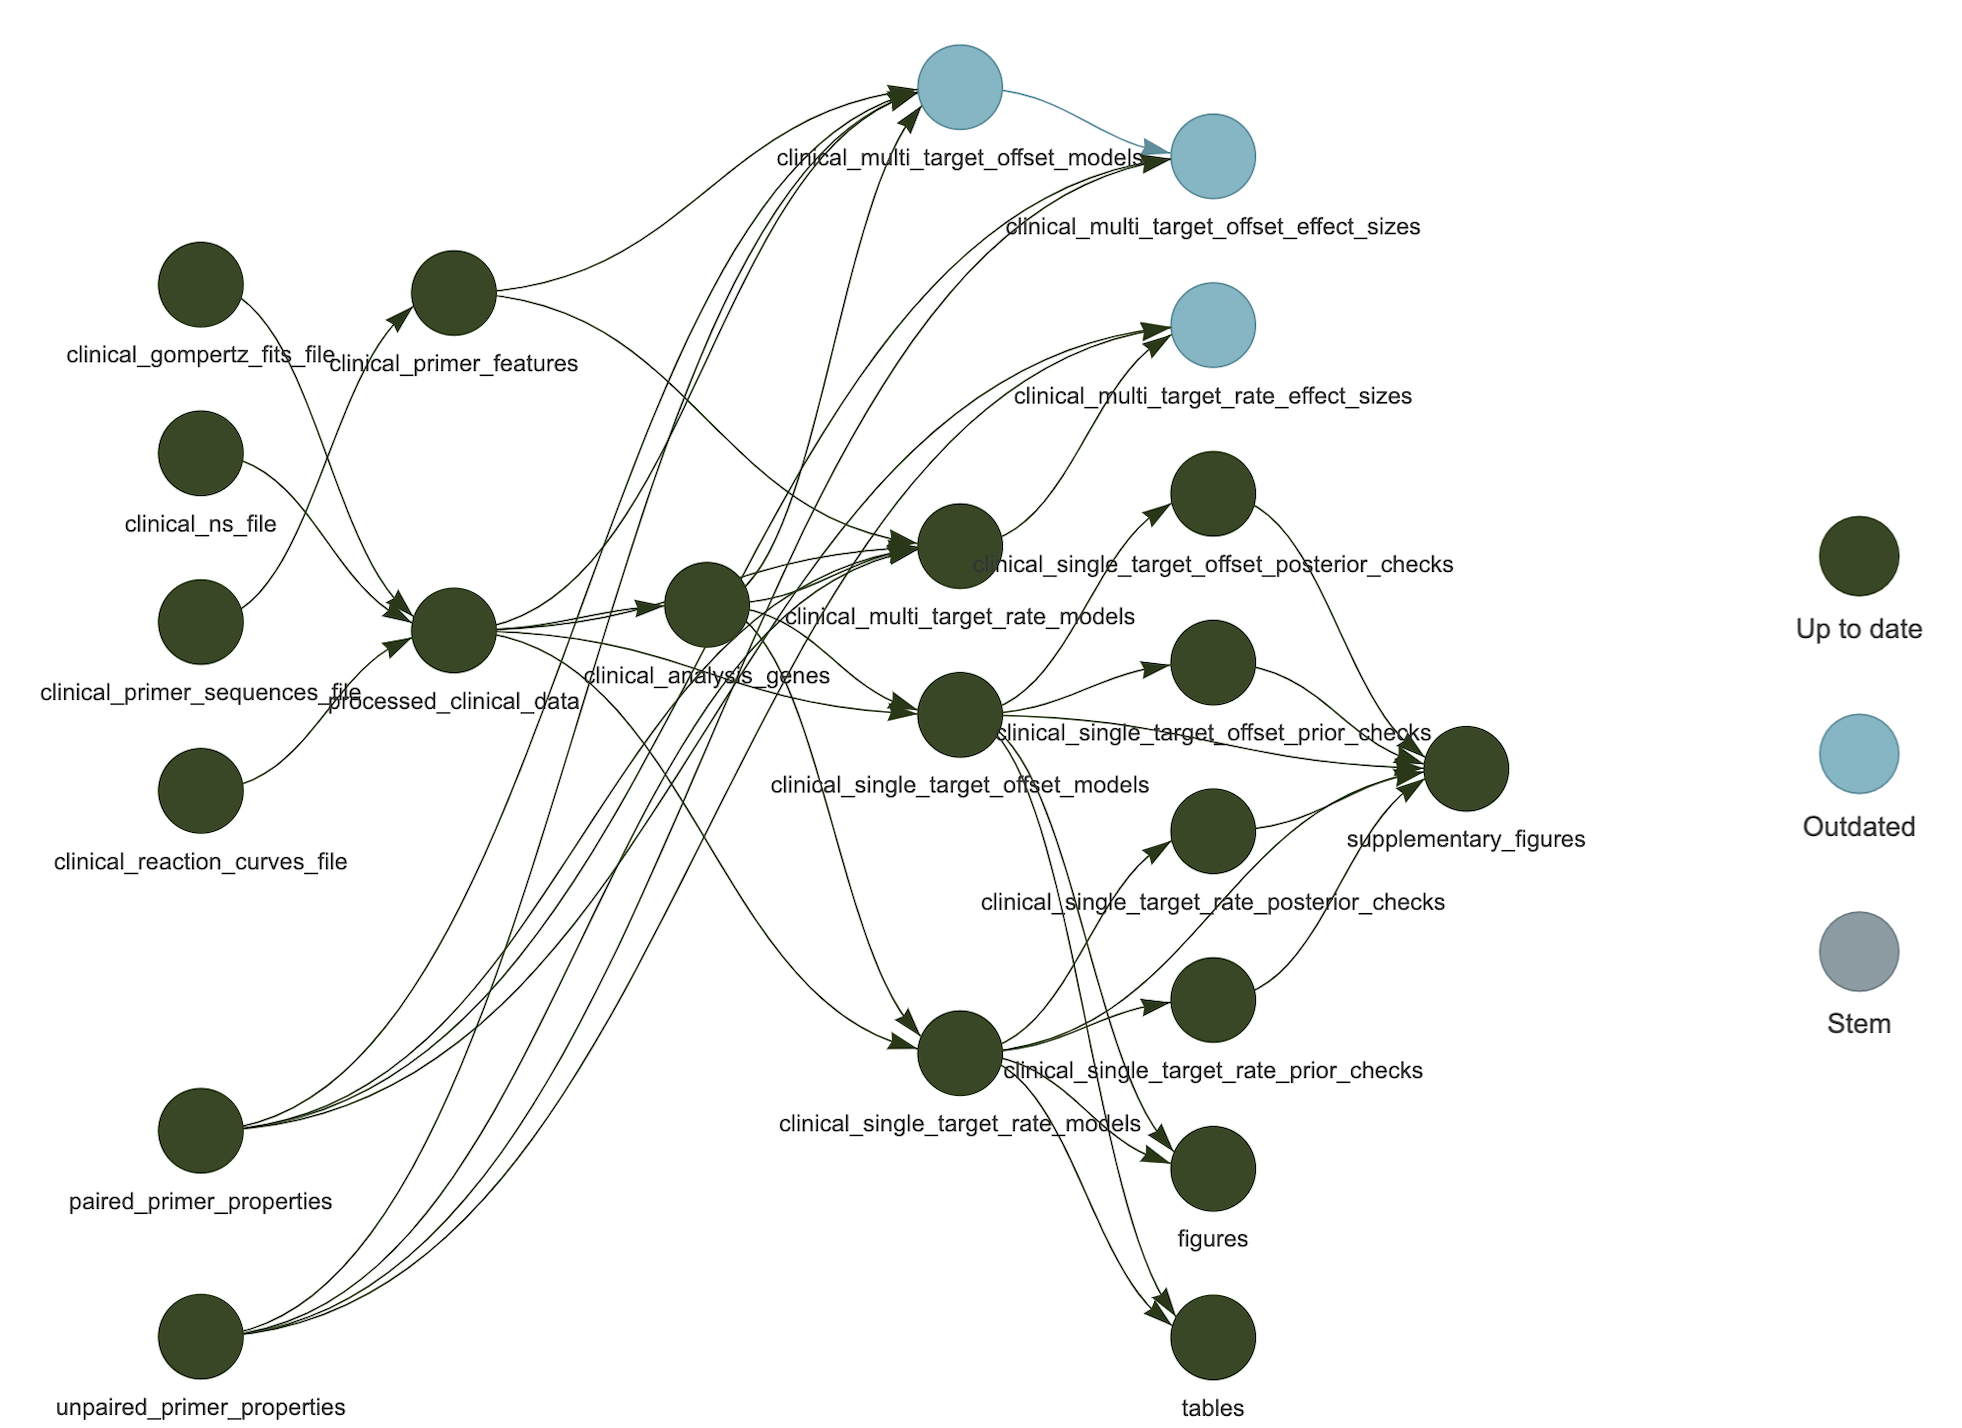
\includegraphics[width=\textwidth]{figures/misc/targets_before_change.png}
    \caption{An example (partially complete) targets dependency graph for the LAMP analysis project in Chapter~2.}
    \label{fig:targets_before_change}
\end{figure}

\subsection{Running and tracking analyses}
The dependency graph as described is useful for ensuring an analysis is modular and flexible (any function for moving from one target to another can be investigated, tweaked or replaced), but also entirely reproducible. At any point, all targets can be completely updated by running \lstinline{targets::tar_make()}. Furthermore, \texttt{targets} is a fantastic resource for tracking the current status of a project (particularly when some constituent processes take a long time). Note that in Figure~\ref{fig:tagets_before_change}, some nodes are blue while others are grey. Blue nodes here indicate a portion of the analysis that has not yet been performed. We are able to automatically track whether any targets need re-running (or running for the first time) via a system of hashes of objects and relating functions. For example, upon altered a preprocessing function for clinical data, we arrive at the dependency graph shown in Figure~\ref{fig:tagets_after_change}. The node corresponding to this altered preprocessed data and all its downstream children are now due for updating the next time \lstinline{targets::tar_make()} is run.

\begin{figure}
    \centering
    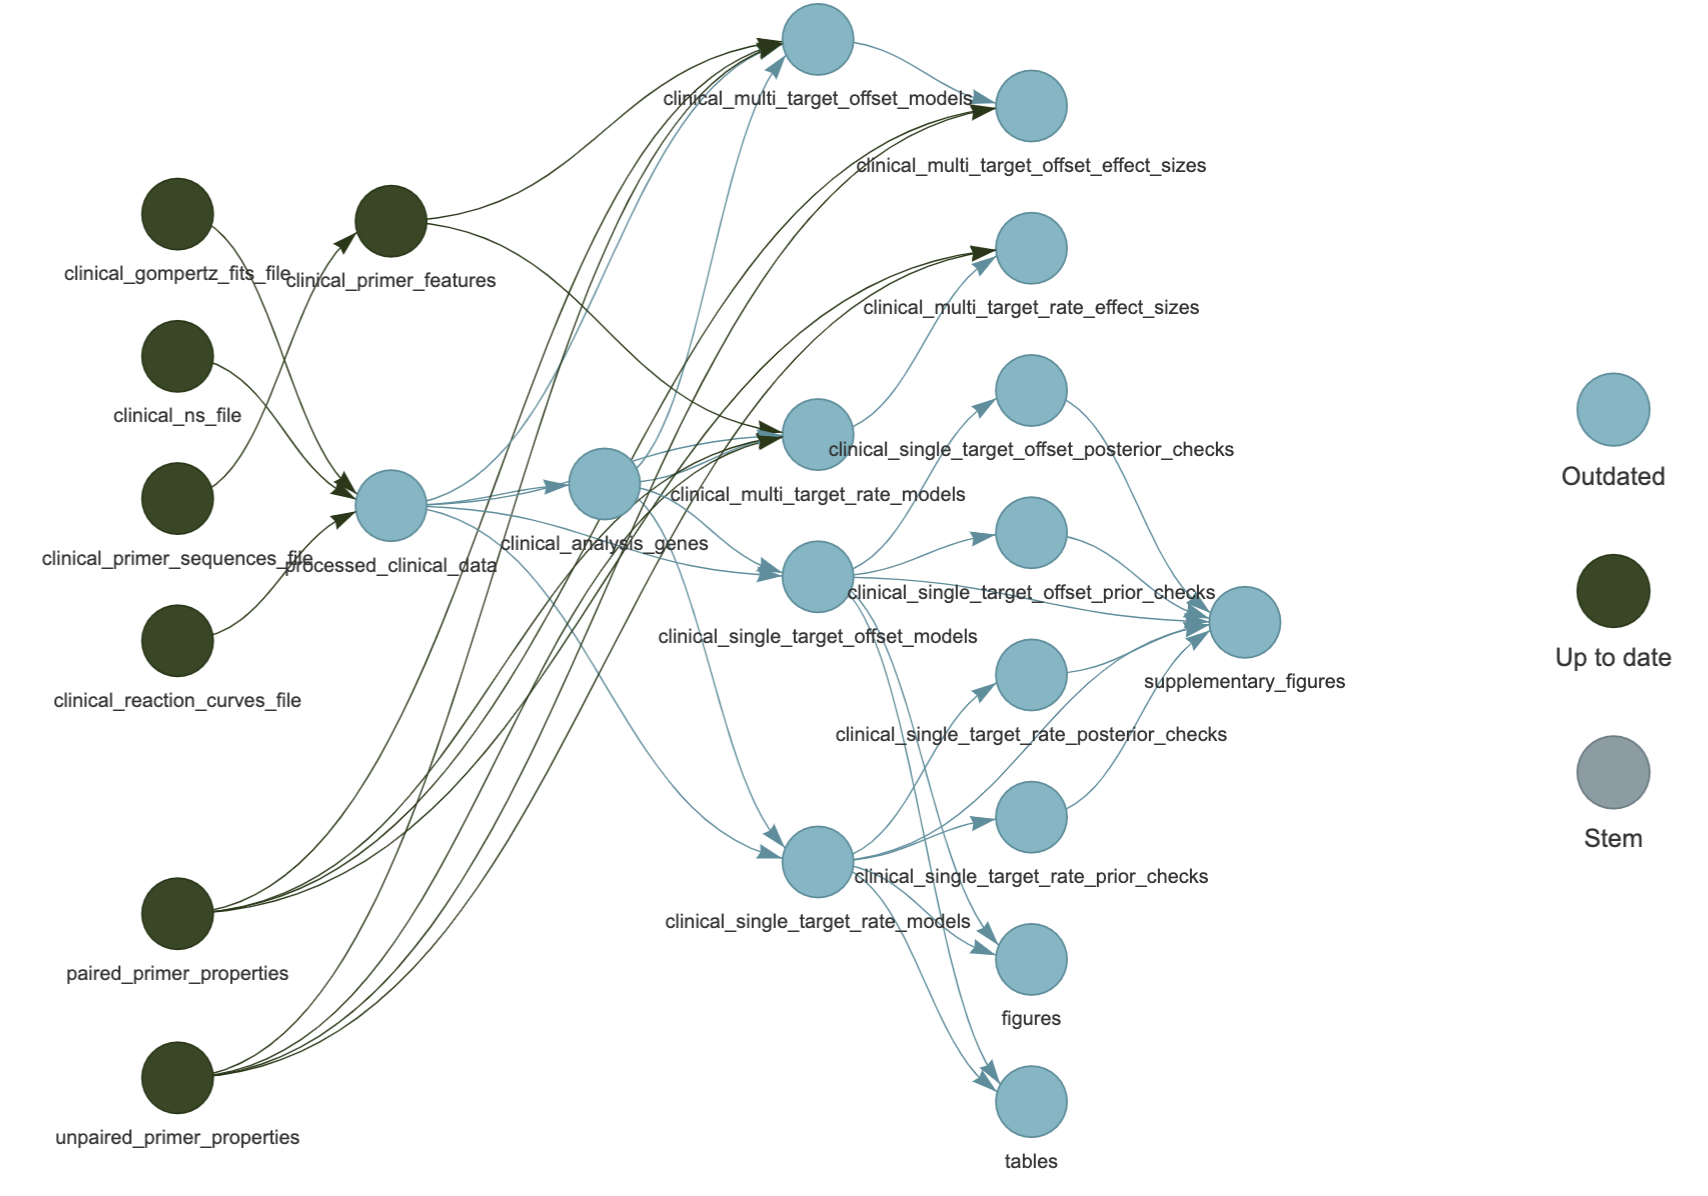
\includegraphics[width=\textwidth]{figures/misc/targets_after_change.png}
    \caption{An example (partially complete) targets dependency graph for the LAMP analysis project in Chapter~2, after changes have been made to a preprocessing step.}
    \label{fig:tagets_after_change}
\end{figure}

\dobib % renders bibliography (only when compiling for chapter only)
 
\end{document}